% Options for packages loaded elsewhere
\PassOptionsToPackage{unicode}{hyperref}
\PassOptionsToPackage{hyphens}{url}
%
\documentclass[
  english,
  man, fleqn, noextraspace]{apa6}
\usepackage{lmodern}
\usepackage{amssymb,amsmath}
\usepackage{ifxetex,ifluatex}
\ifnum 0\ifxetex 1\fi\ifluatex 1\fi=0 % if pdftex
  \usepackage[T1]{fontenc}
  \usepackage[utf8]{inputenc}
  \usepackage{textcomp} % provide euro and other symbols
\else % if luatex or xetex
  \usepackage{unicode-math}
  \defaultfontfeatures{Scale=MatchLowercase}
  \defaultfontfeatures[\rmfamily]{Ligatures=TeX,Scale=1}
\fi
% Use upquote if available, for straight quotes in verbatim environments
\IfFileExists{upquote.sty}{\usepackage{upquote}}{}
\IfFileExists{microtype.sty}{% use microtype if available
  \usepackage[]{microtype}
  \UseMicrotypeSet[protrusion]{basicmath} % disable protrusion for tt fonts
}{}
\makeatletter
\@ifundefined{KOMAClassName}{% if non-KOMA class
  \IfFileExists{parskip.sty}{%
    \usepackage{parskip}
  }{% else
    \setlength{\parindent}{0pt}
    \setlength{\parskip}{6pt plus 2pt minus 1pt}}
}{% if KOMA class
  \KOMAoptions{parskip=half}}
\makeatother
\usepackage{xcolor}
\IfFileExists{xurl.sty}{\usepackage{xurl}}{} % add URL line breaks if available
\IfFileExists{bookmark.sty}{\usepackage{bookmark}}{\usepackage{hyperref}}
\hypersetup{
  pdftitle={EDLD 651 Final Project},
  pdfauthor={Anwesha Guha1, Heidi Iwashita1, Christopher Loan1, Adam Nielsen1, \& Aaron Rothbart1},
  pdflang={en-EN},
  pdfkeywords={keywords},
  hidelinks,
  pdfcreator={LaTeX via pandoc}}
\urlstyle{same} % disable monospaced font for URLs
\usepackage{color}
\usepackage{fancyvrb}
\newcommand{\VerbBar}{|}
\newcommand{\VERB}{\Verb[commandchars=\\\{\}]}
\DefineVerbatimEnvironment{Highlighting}{Verbatim}{commandchars=\\\{\}}
% Add ',fontsize=\small' for more characters per line
\usepackage{framed}
\definecolor{shadecolor}{RGB}{248,248,248}
\newenvironment{Shaded}{\begin{snugshade}}{\end{snugshade}}
\newcommand{\AlertTok}[1]{\textcolor[rgb]{0.94,0.16,0.16}{#1}}
\newcommand{\AnnotationTok}[1]{\textcolor[rgb]{0.56,0.35,0.01}{\textbf{\textit{#1}}}}
\newcommand{\AttributeTok}[1]{\textcolor[rgb]{0.77,0.63,0.00}{#1}}
\newcommand{\BaseNTok}[1]{\textcolor[rgb]{0.00,0.00,0.81}{#1}}
\newcommand{\BuiltInTok}[1]{#1}
\newcommand{\CharTok}[1]{\textcolor[rgb]{0.31,0.60,0.02}{#1}}
\newcommand{\CommentTok}[1]{\textcolor[rgb]{0.56,0.35,0.01}{\textit{#1}}}
\newcommand{\CommentVarTok}[1]{\textcolor[rgb]{0.56,0.35,0.01}{\textbf{\textit{#1}}}}
\newcommand{\ConstantTok}[1]{\textcolor[rgb]{0.00,0.00,0.00}{#1}}
\newcommand{\ControlFlowTok}[1]{\textcolor[rgb]{0.13,0.29,0.53}{\textbf{#1}}}
\newcommand{\DataTypeTok}[1]{\textcolor[rgb]{0.13,0.29,0.53}{#1}}
\newcommand{\DecValTok}[1]{\textcolor[rgb]{0.00,0.00,0.81}{#1}}
\newcommand{\DocumentationTok}[1]{\textcolor[rgb]{0.56,0.35,0.01}{\textbf{\textit{#1}}}}
\newcommand{\ErrorTok}[1]{\textcolor[rgb]{0.64,0.00,0.00}{\textbf{#1}}}
\newcommand{\ExtensionTok}[1]{#1}
\newcommand{\FloatTok}[1]{\textcolor[rgb]{0.00,0.00,0.81}{#1}}
\newcommand{\FunctionTok}[1]{\textcolor[rgb]{0.00,0.00,0.00}{#1}}
\newcommand{\ImportTok}[1]{#1}
\newcommand{\InformationTok}[1]{\textcolor[rgb]{0.56,0.35,0.01}{\textbf{\textit{#1}}}}
\newcommand{\KeywordTok}[1]{\textcolor[rgb]{0.13,0.29,0.53}{\textbf{#1}}}
\newcommand{\NormalTok}[1]{#1}
\newcommand{\OperatorTok}[1]{\textcolor[rgb]{0.81,0.36,0.00}{\textbf{#1}}}
\newcommand{\OtherTok}[1]{\textcolor[rgb]{0.56,0.35,0.01}{#1}}
\newcommand{\PreprocessorTok}[1]{\textcolor[rgb]{0.56,0.35,0.01}{\textit{#1}}}
\newcommand{\RegionMarkerTok}[1]{#1}
\newcommand{\SpecialCharTok}[1]{\textcolor[rgb]{0.00,0.00,0.00}{#1}}
\newcommand{\SpecialStringTok}[1]{\textcolor[rgb]{0.31,0.60,0.02}{#1}}
\newcommand{\StringTok}[1]{\textcolor[rgb]{0.31,0.60,0.02}{#1}}
\newcommand{\VariableTok}[1]{\textcolor[rgb]{0.00,0.00,0.00}{#1}}
\newcommand{\VerbatimStringTok}[1]{\textcolor[rgb]{0.31,0.60,0.02}{#1}}
\newcommand{\WarningTok}[1]{\textcolor[rgb]{0.56,0.35,0.01}{\textbf{\textit{#1}}}}
\usepackage{graphicx,grffile}
\makeatletter
\def\maxwidth{\ifdim\Gin@nat@width>\linewidth\linewidth\else\Gin@nat@width\fi}
\def\maxheight{\ifdim\Gin@nat@height>\textheight\textheight\else\Gin@nat@height\fi}
\makeatother
% Scale images if necessary, so that they will not overflow the page
% margins by default, and it is still possible to overwrite the defaults
% using explicit options in \includegraphics[width, height, ...]{}
\setkeys{Gin}{width=\maxwidth,height=\maxheight,keepaspectratio}
% Set default figure placement to htbp
\makeatletter
\def\fps@figure{htbp}
\makeatother
\setlength{\emergencystretch}{3em} % prevent overfull lines
\providecommand{\tightlist}{%
  \setlength{\itemsep}{0pt}\setlength{\parskip}{0pt}}
\setcounter{secnumdepth}{-\maxdimen} % remove section numbering
% Make \paragraph and \subparagraph free-standing
\ifx\paragraph\undefined\else
  \let\oldparagraph\paragraph
  \renewcommand{\paragraph}[1]{\oldparagraph{#1}\mbox{}}
\fi
\ifx\subparagraph\undefined\else
  \let\oldsubparagraph\subparagraph
  \renewcommand{\subparagraph}[1]{\oldsubparagraph{#1}\mbox{}}
\fi
% Manuscript styling
\usepackage{upgreek}
\captionsetup{font=singlespacing,justification=justified}

% Table formatting
\usepackage{longtable}
\usepackage{lscape}
% \usepackage[counterclockwise]{rotating}   % Landscape page setup for large tables
\usepackage{multirow}		% Table styling
\usepackage{tabularx}		% Control Column width
\usepackage[flushleft]{threeparttable}	% Allows for three part tables with a specified notes section
\usepackage{threeparttablex}            % Lets threeparttable work with longtable

% Create new environments so endfloat can handle them
% \newenvironment{ltable}
%   {\begin{landscape}\begin{center}\begin{threeparttable}}
%   {\end{threeparttable}\end{center}\end{landscape}}
\newenvironment{lltable}{\begin{landscape}\begin{center}\begin{ThreePartTable}}{\end{ThreePartTable}\end{center}\end{landscape}}

% Enables adjusting longtable caption width to table width
% Solution found at http://golatex.de/longtable-mit-caption-so-breit-wie-die-tabelle-t15767.html
\makeatletter
\newcommand\LastLTentrywidth{1em}
\newlength\longtablewidth
\setlength{\longtablewidth}{1in}
\newcommand{\getlongtablewidth}{\begingroup \ifcsname LT@\roman{LT@tables}\endcsname \global\longtablewidth=0pt \renewcommand{\LT@entry}[2]{\global\advance\longtablewidth by ##2\relax\gdef\LastLTentrywidth{##2}}\@nameuse{LT@\roman{LT@tables}} \fi \endgroup}

% \setlength{\parindent}{0.5in}
% \setlength{\parskip}{0pt plus 0pt minus 0pt}

% Overwrite redefinition of paragraph and subparagraph by the default LaTeX template
% See https://github.com/crsh/papaja/issues/292
\makeatletter
\renewcommand{\paragraph}{\@startsection{paragraph}{4}{\parindent}%
  {0\baselineskip \@plus 0.2ex \@minus 0.2ex}%
  {-1em}%
  {\normalfont\normalsize\bfseries\itshape\typesectitle}}

\renewcommand{\subparagraph}[1]{\@startsection{subparagraph}{5}{1em}%
  {0\baselineskip \@plus 0.2ex \@minus 0.2ex}%
  {-\z@\relax}%
  {\normalfont\normalsize\itshape\hspace{\parindent}{#1}\textit{\addperi}}{\relax}}
\makeatother

% \usepackage{etoolbox}
\makeatletter
\patchcmd{\HyOrg@maketitle}
  {\section{\normalfont\normalsize\abstractname}}
  {\section*{\normalfont\normalsize\abstractname}}
  {}{\typeout{Failed to patch abstract.}}
\patchcmd{\HyOrg@maketitle}
  {\section{\protect\normalfont{\@title}}}
  {\section*{\protect\normalfont{\@title}}}
  {}{\typeout{Failed to patch title.}}
\makeatother
\shorttitle{New York City Graduation Outcome by Borough and Student Classification}
\keywords{keywords\newline\indent Word count: X}
\DeclareDelayedFloatFlavor{ThreePartTable}{table}
\DeclareDelayedFloatFlavor{lltable}{table}
\DeclareDelayedFloatFlavor*{longtable}{table}
\makeatletter
\renewcommand{\efloat@iwrite}[1]{\immediate\expandafter\protected@write\csname efloat@post#1\endcsname{}}
\makeatother
\usepackage{lineno}

\linenumbers
\usepackage{csquotes}
\raggedbottom
\setlength{\parskip}{0pt}
\ifxetex
  % Load polyglossia as late as possible: uses bidi with RTL langages (e.g. Hebrew, Arabic)
  \usepackage{polyglossia}
  \setmainlanguage[]{english}
\else
  \usepackage[shorthands=off,main=english]{babel}
\fi

\title{EDLD 651 Final Project}
\author{Anwesha Guha\textsuperscript{1}, Heidi Iwashita\textsuperscript{1}, Christopher Loan\textsuperscript{1}, Adam Nielsen\textsuperscript{1}, \& Aaron Rothbart\textsuperscript{1}}
\date{}


\authornote{

All work done herein represents contributions from all authors equally. Author order is alphabetical.

}

\affiliation{\vspace{0.5cm}\textsuperscript{1} University of Oregon}

\abstract{
FILL IN ABSTRACT IF WANTED
}



\begin{document}
\maketitle

\hypertarget{introduction}{%
\section{Introduction}\label{introduction}}

Now more than ever, it is crucial to address systematic disparities in education. Though there has been modest improvement in recent years (Disability Scoop, 2019), high school graduation rates still are significantly lower in specific groups who have historically received unequal access to resources, in particular students with disabilities and students with limited English proficiency (Burke, 2015). This is especially troubling considering the lower rates of employment among adults who do not complete high school (Schifter, 2016). Approximately 67\% of students receiving special education services in the U.S. obtain their high school diploma, and only 66\% of English learners graduate on time from secondary education (Johnson, 2019; National Center for Education Statistics, n.d.). These percentages fall short of the approximately 85\% of all high school students who graduate (National Center for Education Statistics, n.d.).

In light of these concerns, we decided to explore high school graduation rates for students with disabilities and with limited English proficiency as compared to general education populations. This data can be assessed to identify systematic breakdowns and disparities impacting marginalized student populations. In particular, we wanted to see if the national data was represented regionally by looking at data from New York City schools. Furthermore, to examine the impact of geographical disparities in access to educational resources, this paper will also examine graduation outcomes across New York City boroughs.

\hypertarget{methods}{%
\section{Methods}\label{methods}}

We retrieved data collected by the Department of Education from \href{https://data.cityofnewyork.us/Education/2005-2010-Graduation-Outcomes-By-Borough/avir-tzek}{\emph{NYC OpenData}}(NYC Open Data, 2019). The data contains four-year graduation outcomes for the cohorts of 2001 through 2006 (classes of 2005 - 2010). According to the website, graduates are defined as those students earning either a Local or Regents diploma and exclude those earning either a special education (IEP) diploma or GED. Additionally, students who were in a school for less than five months are not included in the school cohort data. The data was last updated in April 2019.

\hypertarget{participants}{%
\subsection{Participants}\label{participants}}

The original dataset of high school students contained 22 variables and 385 rows.

First, we import and clean our data to begin our analyses using the \texttt{import()} and \texttt{here()} functions from \texttt{rio} and \texttt{here} packages.

\hypertarget{pivots}{%
\subsection{Pivots}\label{pivots}}

The data we are starting with are already tidy, but for the purposes of demonstrating our rather acute proficiency in our \emph{ability} to tidy data, in this segment will make the data untidy and then tidy it once more.

\begin{Shaded}
\begin{Highlighting}[]
\NormalTok{messy_grad <-}\StringTok{ }\NormalTok{grad }\OperatorTok\StringTok{ }
\StringTok{  }\KeywordTok{pivot_wider}\NormalTok{(}\DataTypeTok{names_from =}\NormalTok{ borough,}
              \DataTypeTok{values_from =}\NormalTok{ total_cohort)}

\NormalTok{clean_grad <-}\StringTok{ }\NormalTok{messy_grad }\OperatorTok\StringTok{ }
\StringTok{  }\KeywordTok{pivot_longer}\NormalTok{(}\DataTypeTok{cols =} \KeywordTok{c}\NormalTok{(}\StringTok{"Bronx"}\OperatorTok{:}\StringTok{"Staten Island"}\NormalTok{),}
               \DataTypeTok{names_to =} \StringTok{"borough"}\NormalTok{,}
               \DataTypeTok{values_to =} \StringTok{"total_cohort"}\NormalTok{,}
               \DataTypeTok{values_drop_na =} \OtherTok{TRUE}\NormalTok{)}

\NormalTok{clean_grad <-}\StringTok{ }\NormalTok{clean_grad[, }\KeywordTok{c}\NormalTok{(}\DecValTok{1}\NormalTok{,}\DecValTok{21}\NormalTok{,}\DecValTok{2}\NormalTok{,}\DecValTok{22}\NormalTok{,}\DecValTok{3}\OperatorTok{:}\DecValTok{20}\NormalTok{)]}
\end{Highlighting}
\end{Shaded}

After tidying the entire dataset, we can focus on our variables of interest: enrollment and graduation outcomes for specific boroughs, cohort years and student classifications.

Through this re-coding, and the variables recorded for each, we find that each graduation outcome category (number graduated, dropped out, still enrolled) do not sum to the total number of students in the cohort. This made clear the data was not as tidy as it initially seemed.

As shown above, we mutated the data to create a new column named \texttt{unclassified\_n}, which holds the number of students in each level that are unaccounted for.

We can see those results visually here, first by student classification:

\begin{tabular}{l|r|r|r|r}
\hline
student\_characteristic & mean\_grad\_pct & mean\_dropout\_pct & mean\_enrolled\_pct & mean\_unclassified\_pct\\
\hline
ELL & 34.23714 & 23.10286 & 36.58571 & 6.082857\\
\hline
EP & 61.58000 & 11.98000 & 23.31714 & 3.125714\\
\hline
SPED & 24.74857 & 23.24000 & 37.77714 & 14.242857\\
\hline
Non-SPED & 64.27143 & 11.53714 & 22.56571 & 1.625714\\
\hline
\end{tabular}

.

The table shows that, of the student classifications, the SPED classification contains the largest percentage of unclassified students at roughly 14\%. Notably, 6\% of students with ELL classification also are also unclassified, compared to 3\% of English proficient students.

We also examine outcomes by borough here:

\begin{tabular}{l|r|r|r|r|r}
\hline
borough & mean\_local & mean\_grad\_pct & mean\_dropout\_pct & mean\_enrolled\_pct & mean\_unclassified\_pct\\
\hline
Bronx & 17.38571 & 40.28571 & 20.38214 & 31.38214 & 7.967857\\
\hline
Brooklyn & 14.71429 & 42.75714 & 18.38929 & 33.10000 & 5.750000\\
\hline
Manhattan & 15.38929 & 47.38214 & 16.79643 & 30.05357 & 5.767857\\
\hline
Queens & 14.70714 & 46.96429 & 17.94286 & 29.92500 & 5.175000\\
\hline
Staten Island & 16.89643 & 53.65714 & 13.81429 & 25.84643 & 6.685714\\
\hline
\end{tabular}

.

These unclassified students were not concentrated in any one year, shown in the table here:

\begin{tabular}{r|r|r|r|r|r}
\hline
cohort & mean\_local & mean\_grad\_pct & mean\_dropout\_pct & mean\_enrolled\_pct & mean\_unclassified\_pct\\
\hline
2001 & 17.805 & 41.360 & 21.8100 & 29.4950 & 7.365\\
\hline
2002 & 16.015 & 40.005 & 20.4750 & 33.2950 & 6.225\\
\hline
2003 & 15.130 & 41.555 & 18.1950 & 35.3800 & 4.880\\
\hline
2004 & 16.080 & 45.485 & 16.5700 & 32.6100 & 5.340\\
\hline
2005 & 15.770 & 48.520 & 15.0100 & 29.0750 & 7.385\\
\hline
2006 & 14.965 & 53.270 & 15.0975 & 25.2875 & 6.345\\
\hline
\end{tabular}

.

Additional use of the \texttt{pivot\_longer()} function allowed us to further tidy the data to create a \textbf{graduation outcomes} variable, so we could see the average percentage of students for each graduation outcome, by student classification (see Figure 1).

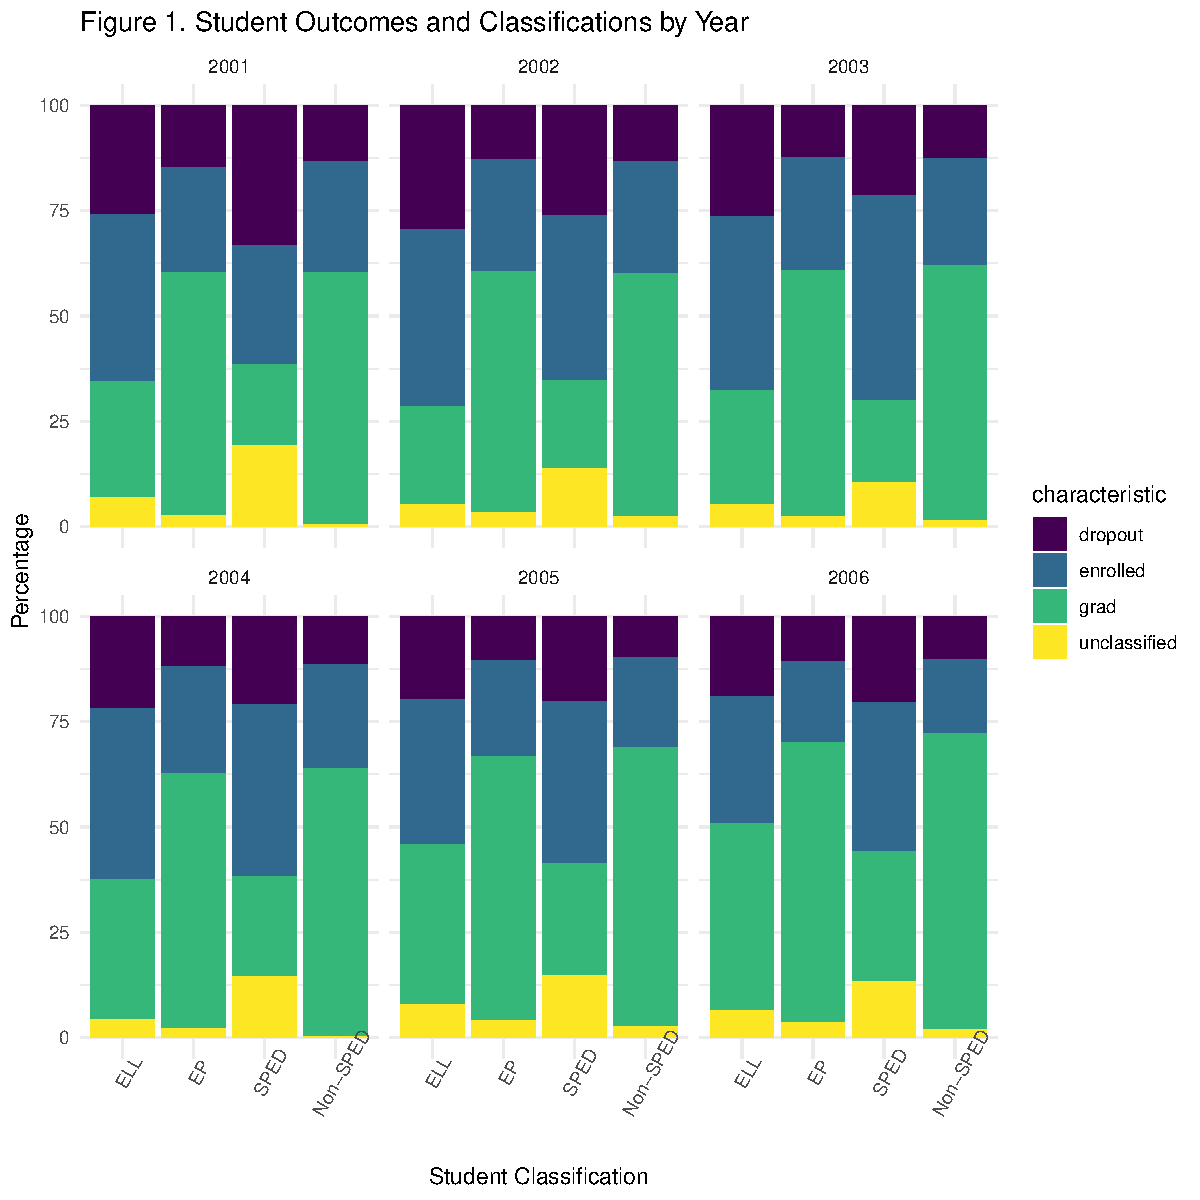
\includegraphics{EDLD_651_Final_Project_Draft_files/figure-latex/descriptives_of_dataset-1.pdf}

\hypertarget{data-analysis}{%
\subsection{Data analysis}\label{data-analysis}}

All analysis were conducted in R, with heavy reliance upon the \texttt{\{tidyverse\}} packages to manipulate and visualize the data.
We used the following R versions and packages for this project:
R (Version 4.0.2; R Core Team, 2020) and the R-packages \emph{dplyr} (Version 1.0.2; Wickham et al., 2020), \emph{forcats} (Version 0.5.0; Wickham, 2020a), \emph{ggplot2} (Version 3.3.2; Wickham, 2016), \emph{here} (Version 1.0.0; Müller, 2017), \emph{janitor} (Version 2.0.1; Firke, 2020), \emph{kableExtra} (Version 1.3.1; Zhu, 2020), \emph{knitr} (Version 1.30; Xie, 2015), \emph{papaja} (Version 0.1.0.9997; Aust \& Barth, 2020), \emph{purrr} (Version 0.3.4; Henry \& Wickham, 2020), \emph{readr} (Version 1.4.0; Wickham, Hester, \& Francois, 2018), \emph{rio} (Version 0.5.16; Chan, Chan, Leeper, \& Becker, 2018), \emph{stringr} (Version 1.4.0; Wickham, 2019), \emph{tibble} (Version 3.0.4; Müller \& Wickham, 2020), \emph{tidyr} (Version 1.1.2; Wickham, 2020b), and \emph{tidyverse} (Version 1.3.0; Wickham, Averick, et al., 2019).

\hypertarget{results}{%
\section{Results}\label{results}}

Visual inspection of Figure 2 demonstrates heterogeneity in the gaps between ELL and EP students. Certain Boroughs (e.g., Staten Island) have much larger gaps between proficiency than others (e.g., Brooklyn). This is most easily seen from difference in the dashed lines which represent the means of each group within a given Borough.

From an equity framework, it is concerning that this gap is not equal across boroughs. Ideally, any difference in graduation based on EL status between students would be constant despite location. Without follow-ups to gather more qualitative (or highly dimensional quantitative) data, it is difficult to explain why Boroughs with higher EP graduation rates do not have correspondingly higher ELL graduation rates.

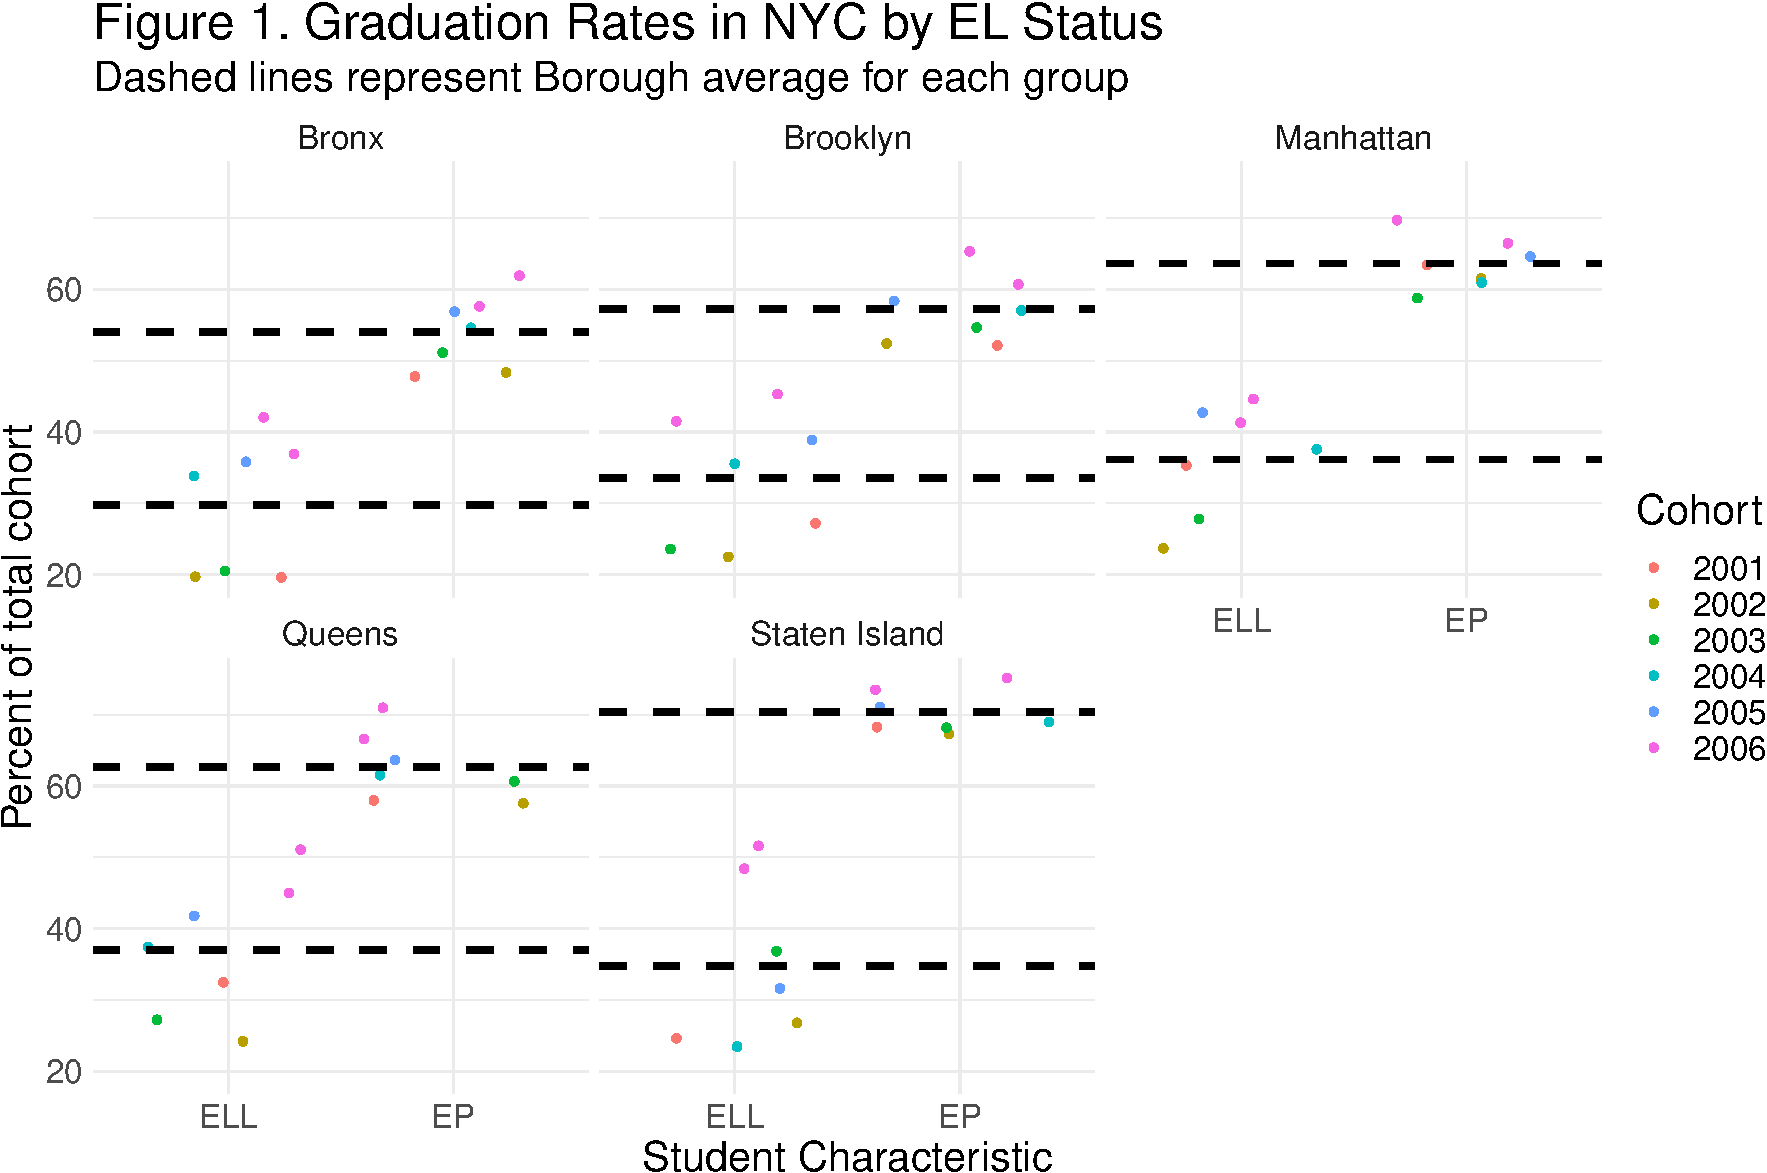
\includegraphics{EDLD_651_Final_Project_Draft_files/figure-latex/graph_results_EL_graph-1.pdf}

Visual inspection of Figure 3 suggests less variability in the difference between average graduation rates of SPED vs.~non-SPED students across Boroughs. Unlike ELL vs.~EP students, SPED students appear to succeed at rates relative to their Borough. This may suggest support for SPED students increases proportionately to non-SPED students, which is essential from an equity framework.

This trend is evident when we compare the difference between these groups across districts (e.g., Staten Island \& Manhattan) which perform well. Visually this looks like a shift in both mean lines, rather than in increase only for non-SPED students.

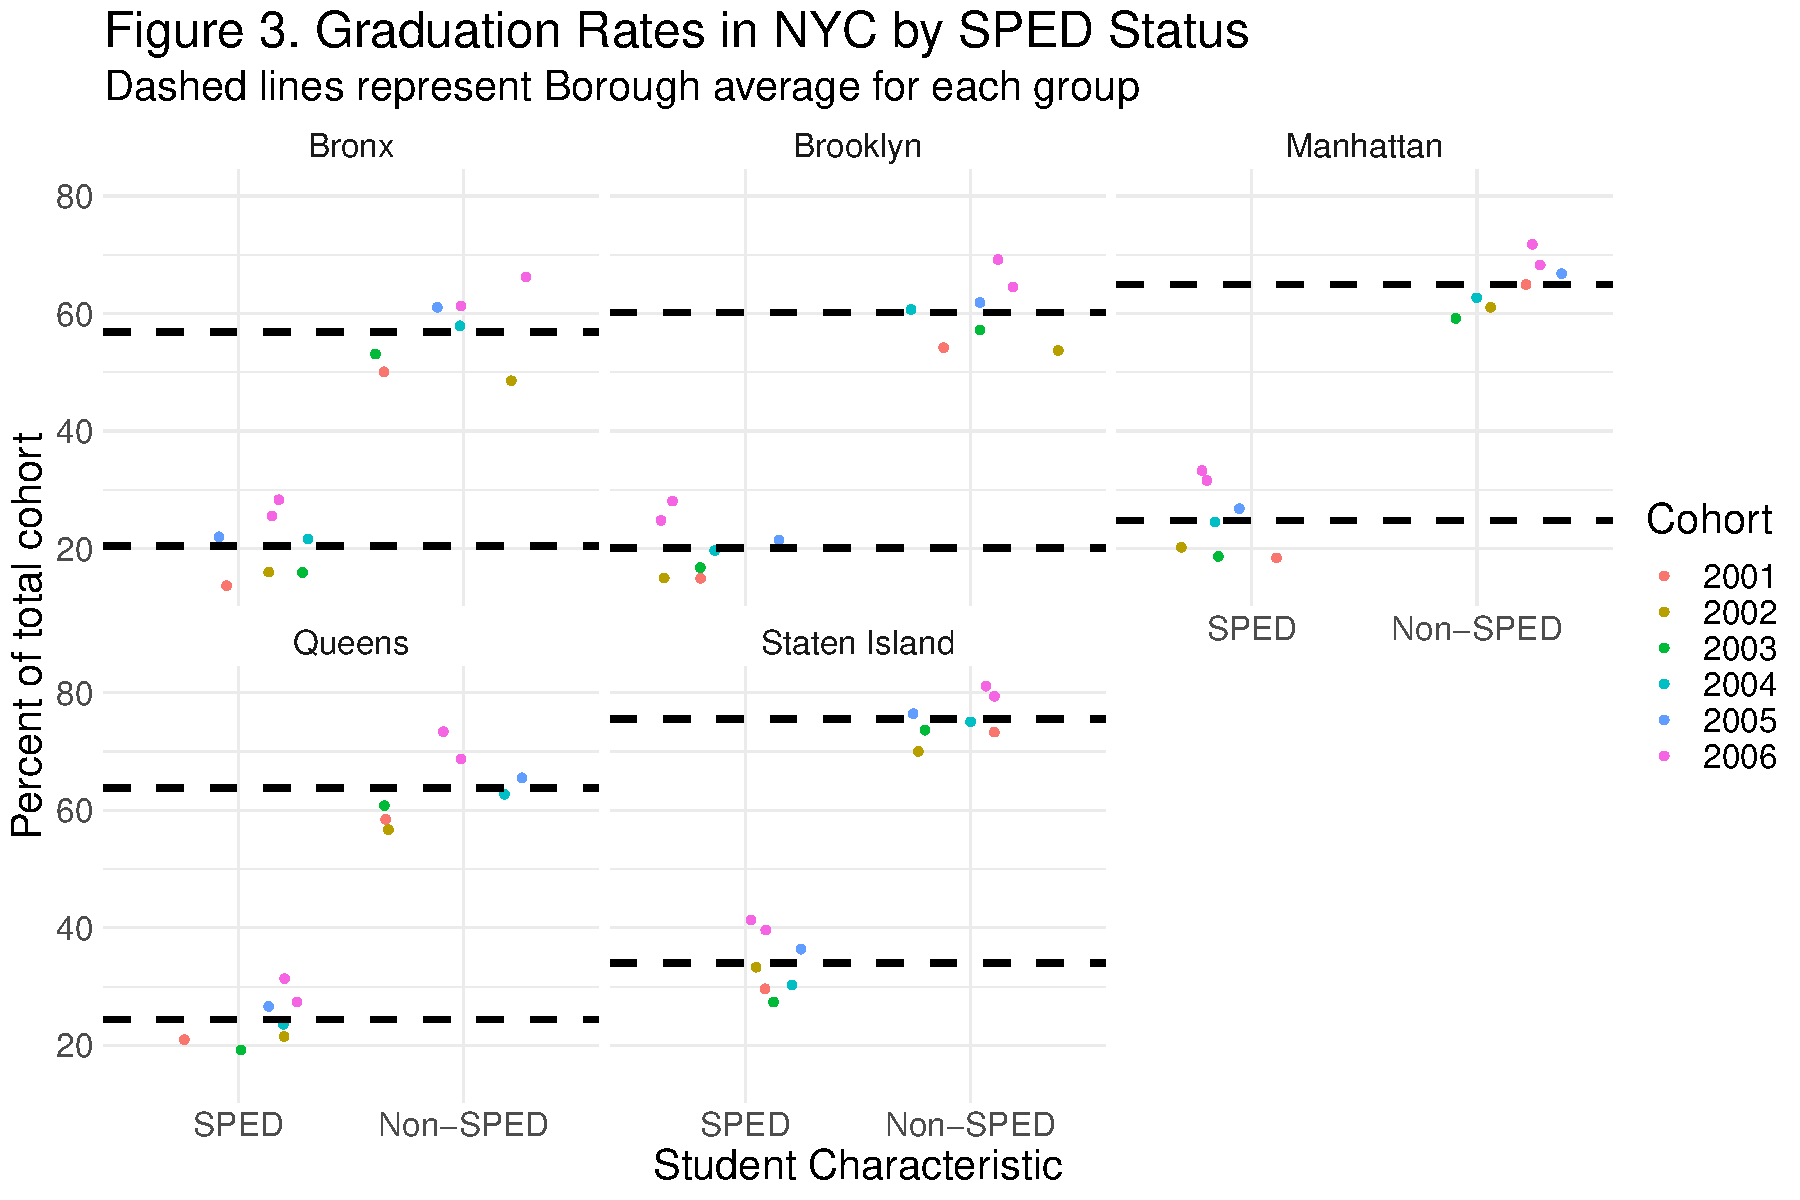
\includegraphics{EDLD_651_Final_Project_Draft_files/figure-latex/graph_results_SPED-1.pdf}

For in both visual analyses------though some variability over years is evident------annual differences are much smaller than the differences between groups (and in some cases differences between Boroughs). Overall, though, graduation rates seem to not be too different over time for either group comparison.

\hypertarget{discussion}{%
\section{Discussion}\label{discussion}}

This project leveraged public data to determine differential graduation outcomes across student classification status. Specifically, we compared differences between (i) ELL and EP as well as (ii) SPED and non-SPED across boroughs. We incorporated several years of data and visualized these as a jittered scatter plot with mean lines at each Borough and student-classification Cluster to clearly identify differences between groups.

As this was a purely descriptive analysis, we recommend inferential statistics to explore the significance of these group differences. Furthermore, we suggest future research incorporate experts and educational theorists with the purpose of explaining these differences. Through greater explanation and exploration, we hope differences in support for ELL vs.~EP students across borough can be minimized in a way that all students are supported adequately.

We pose a few considerations in an exploration of potentially confounding variables which explain the variation in these averages (particularly for ELL/EP). These include but are not limited to: unequal access to resources by all portions of the school, percent of teachers that speak languages other than English, predominant non-English language(s) is/are spoken in each borough, Average qualification of SPED/ELL teachers, and parental access to (and leverage of) extra-curricular educational resources.

\newpage

\hypertarget{references}{%
\section{References}\label{references}}

\begingroup
\setlength{\parindent}{-0.5in}
\setlength{\leftskip}{0.5in}

\hypertarget{refs}{}
\leavevmode\hypertarget{ref-R-papaja}{}%
Aust, F., \& Barth, M. (2020). \emph{papaja: Create APA manuscripts with R Markdown}. Retrieved from \url{https://github.com/crsh/papaja}

\leavevmode\hypertarget{ref-burke2015early}{}%
Burke, A. (2015). Early identification of high school graduation outcomes in oregon leadership network schools. \emph{Regional Educational Laboratory Northwest}.

\leavevmode\hypertarget{ref-R-rio}{}%
Chan, C.-h., Chan, G. C., Leeper, T. J., \& Becker, J. (2018). \emph{Rio: A swiss-army knife for data file i/o}.

\leavevmode\hypertarget{ref-Graduati54:online}{}%
Disability Scoop. (2019). \emph{Graduation rate for students with disabilities shows improvement}. \url{https://www.disabilityscoop.com/2019/01/30/graduation-rate-shows-improvement/25962/\#:~:text=For\%20the\%202016\%2D2017\%20school,that\%20the\%20rate\%20has\%20increased.}

\leavevmode\hypertarget{ref-R-janitor}{}%
Firke, S. (2020). \emph{Janitor: Simple tools for examining and cleaning dirty data}. Retrieved from \url{https://CRAN.R-project.org/package=janitor}

\leavevmode\hypertarget{ref-R-purrr}{}%
Henry, L., \& Wickham, H. (2020). \emph{Purrr: Functional programming tools}. Retrieved from \url{https://CRAN.R-project.org/package=purrr}

\leavevmode\hypertarget{ref-johnson2019effects}{}%
Johnson, A. (2019). The effects of english learner classification on high school graduation and college attendance. \emph{AERA Open}, \emph{5}(2), 2332858419850801.

\leavevmode\hypertarget{ref-R-here}{}%
Müller, K. (2017). \emph{Here: A simpler way to find your files}. Retrieved from \url{https://CRAN.R-project.org/package=here}

\leavevmode\hypertarget{ref-R-tibble}{}%
Müller, K., \& Wickham, H. (2020). \emph{Tibble: Simple data frames}. Retrieved from \url{https://CRAN.R-project.org/package=tibble}

\leavevmode\hypertarget{ref-Table1Pu71:online}{}%
National Center for Education Statistics. (n.d.). \emph{Table 1. Public high school 4-year adjusted cohort graduation rate (acgr), by race/ethnicity and selected demographic characteristics for the united states, the 50 states, and the district of columbia: School year 2016--17}. \url{https://nces.ed.gov/ccd/tables/ACGR_RE_and_characteristics_2016-17.asp}.

\leavevmode\hypertarget{ref-2005201053:online}{}%
NYC Open Data. (2019). \emph{2005-2010 graduation outcomes - by borough}. \url{https://data.cityofnewyork.us/Education/2005-2010-Graduation-Outcomes-By-Borough/avir-tzek}.

\leavevmode\hypertarget{ref-R-base}{}%
R Core Team. (2020). \emph{R: A language and environment for statistical computing}. Vienna, Austria: R Foundation for Statistical Computing. Retrieved from \url{https://www.R-project.org/}

\leavevmode\hypertarget{ref-schifter2016using}{}%
Schifter, L. A. (2016). Using survival analysis to understand graduation of students with disabilities. \emph{Exceptional Children}, \emph{82}(4), 479--496.

\leavevmode\hypertarget{ref-R-ggplot2}{}%
Wickham, H. (2016). \emph{Ggplot2: Elegant graphics for data analysis}. Springer-Verlag New York. Retrieved from \url{https://ggplot2.tidyverse.org}

\leavevmode\hypertarget{ref-R-stringr}{}%
Wickham, H. (2019). \emph{Stringr: Simple, consistent wrappers for common string operations}. Retrieved from \url{https://CRAN.R-project.org/package=stringr}

\leavevmode\hypertarget{ref-R-forcats}{}%
Wickham, H. (2020a). \emph{Forcats: Tools for working with categorical variables (factors)}. Retrieved from \url{https://CRAN.R-project.org/package=forcats}

\leavevmode\hypertarget{ref-R-tidyr}{}%
Wickham, H. (2020b). \emph{Tidyr: Tidy messy data}. Retrieved from \url{https://CRAN.R-project.org/package=tidyr}

\leavevmode\hypertarget{ref-R-tidyverse}{}%
Wickham, H., Averick, M., Bryan, J., Chang, W., McGowan, L. D., François, R., \ldots{} Yutani, H. (2019). Welcome to the tidyverse. \emph{Journal of Open Source Software}, \emph{4}(43), 1686. \url{https://doi.org/10.21105/joss.01686}

\leavevmode\hypertarget{ref-R-dplyr}{}%
Wickham, H., François, R., Henry, L., \& Müller, K. (2020). \emph{Dplyr: A grammar of data manipulation}. Retrieved from \url{https://CRAN.R-project.org/package=dplyr}

\leavevmode\hypertarget{ref-R-readr}{}%
Wickham, H., Hester, J., \& Francois, R. (2018). \emph{Readr: Read rectangular text data}. Retrieved from \url{https://CRAN.R-project.org/package=readr}

\leavevmode\hypertarget{ref-R-knitr}{}%
Xie, Y. (2015). \emph{Dynamic documents with R and knitr} (2nd ed.). Boca Raton, Florida: Chapman; Hall/CRC. Retrieved from \url{https://yihui.org/knitr/}

\leavevmode\hypertarget{ref-R-kableExtra}{}%
Zhu, H. (2020). \emph{KableExtra: Construct complex table with 'kable' and pipe syntax}. Retrieved from \url{https://CRAN.R-project.org/package=kableExtra}

\endgroup


\end{document}
